\section{Discussion: Coupled Variables and Limits}
\label{sec:discussion}

The literature supports a coupled rather than linear interpretation of LLZO processing. Lithium inventory affects phase formation and volatilization; the thermal path converts that inventory into a density and boundary state; the boundary state controls how the bulk response appears in impedance and how current is distributed at a Li interface. Reviews that separate “materials,” “processing” and “battery” sections are useful for navigation, but the same specimen-level variables cross those boundaries \cite{cao2019modeling,wang2020garnet,wang2024accelerating,zhao2024review}.

Three recurring tensions explain much of the apparent disagreement. First, lithium excess can promote phase purity yet increase volatilization or carbonate formation when cover geometry and exposure are not matched \cite{heywood2023tailoring,gullbrekken2025phase,montoya2024lithium,shi2025li2co3}. Second, a transient liquid or glassy boundary can improve densification and lower grain-boundary resistance while changing mechanical compliance or electronic leakage \cite{luo2019influence,park2026li2co3,yao2026elimination}. Third, rapid heating can preserve a fine microstructure and reduce furnace time but create gradients in temperature, lithium retention and surface chemistry \cite{aman2026susceptor,ramos2026ultrafast,zhang2024unveiling}.

These tensions make a universal “best route” claim scientifically weak. A stronger statement is conditional: a route is favorable for a target form factor when it reaches a specified phase fraction and density with a measured lithium inventory, produces a characterized boundary, and retains a defined conductivity under a reproducible geometry. The same criteria also make negative results useful because they identify which variable prevented transfer.

\subsection{A practical comparison matrix}

For each paper, the reader can reconstruct the following chain: precursor and lithium source $\rightarrow$ green density and thickness $\rightarrow$ calcination and sintering atmosphere $\rightarrow$ phase fraction and retained composition $\rightarrow$ density, grains and boundaries $\rightarrow$ bulk, boundary and total resistance $\rightarrow$ Li or cathode cell response. Missing links should be marked as not reported rather than silently inferred. This matrix operationalizes the minimum-record contribution and aligns with recent calls for scalable LLZO processing and standardized interface tests \cite{wang2024accelerating,touidjine2026tapex,klimpel2023standardizing}.

Figure~\ref{fig:coupled-variables} makes the feedback structure explicit. Chemistry and thermal history set phase and density; boundaries and surfaces then mediate the measured bulk, grain-boundary and total responses. Measurement conditions feed back into process design because an apparent conductivity gain can disappear when geometry, pressure or uncertainty are standardized.

\begin{figure}[t]
  \centering
  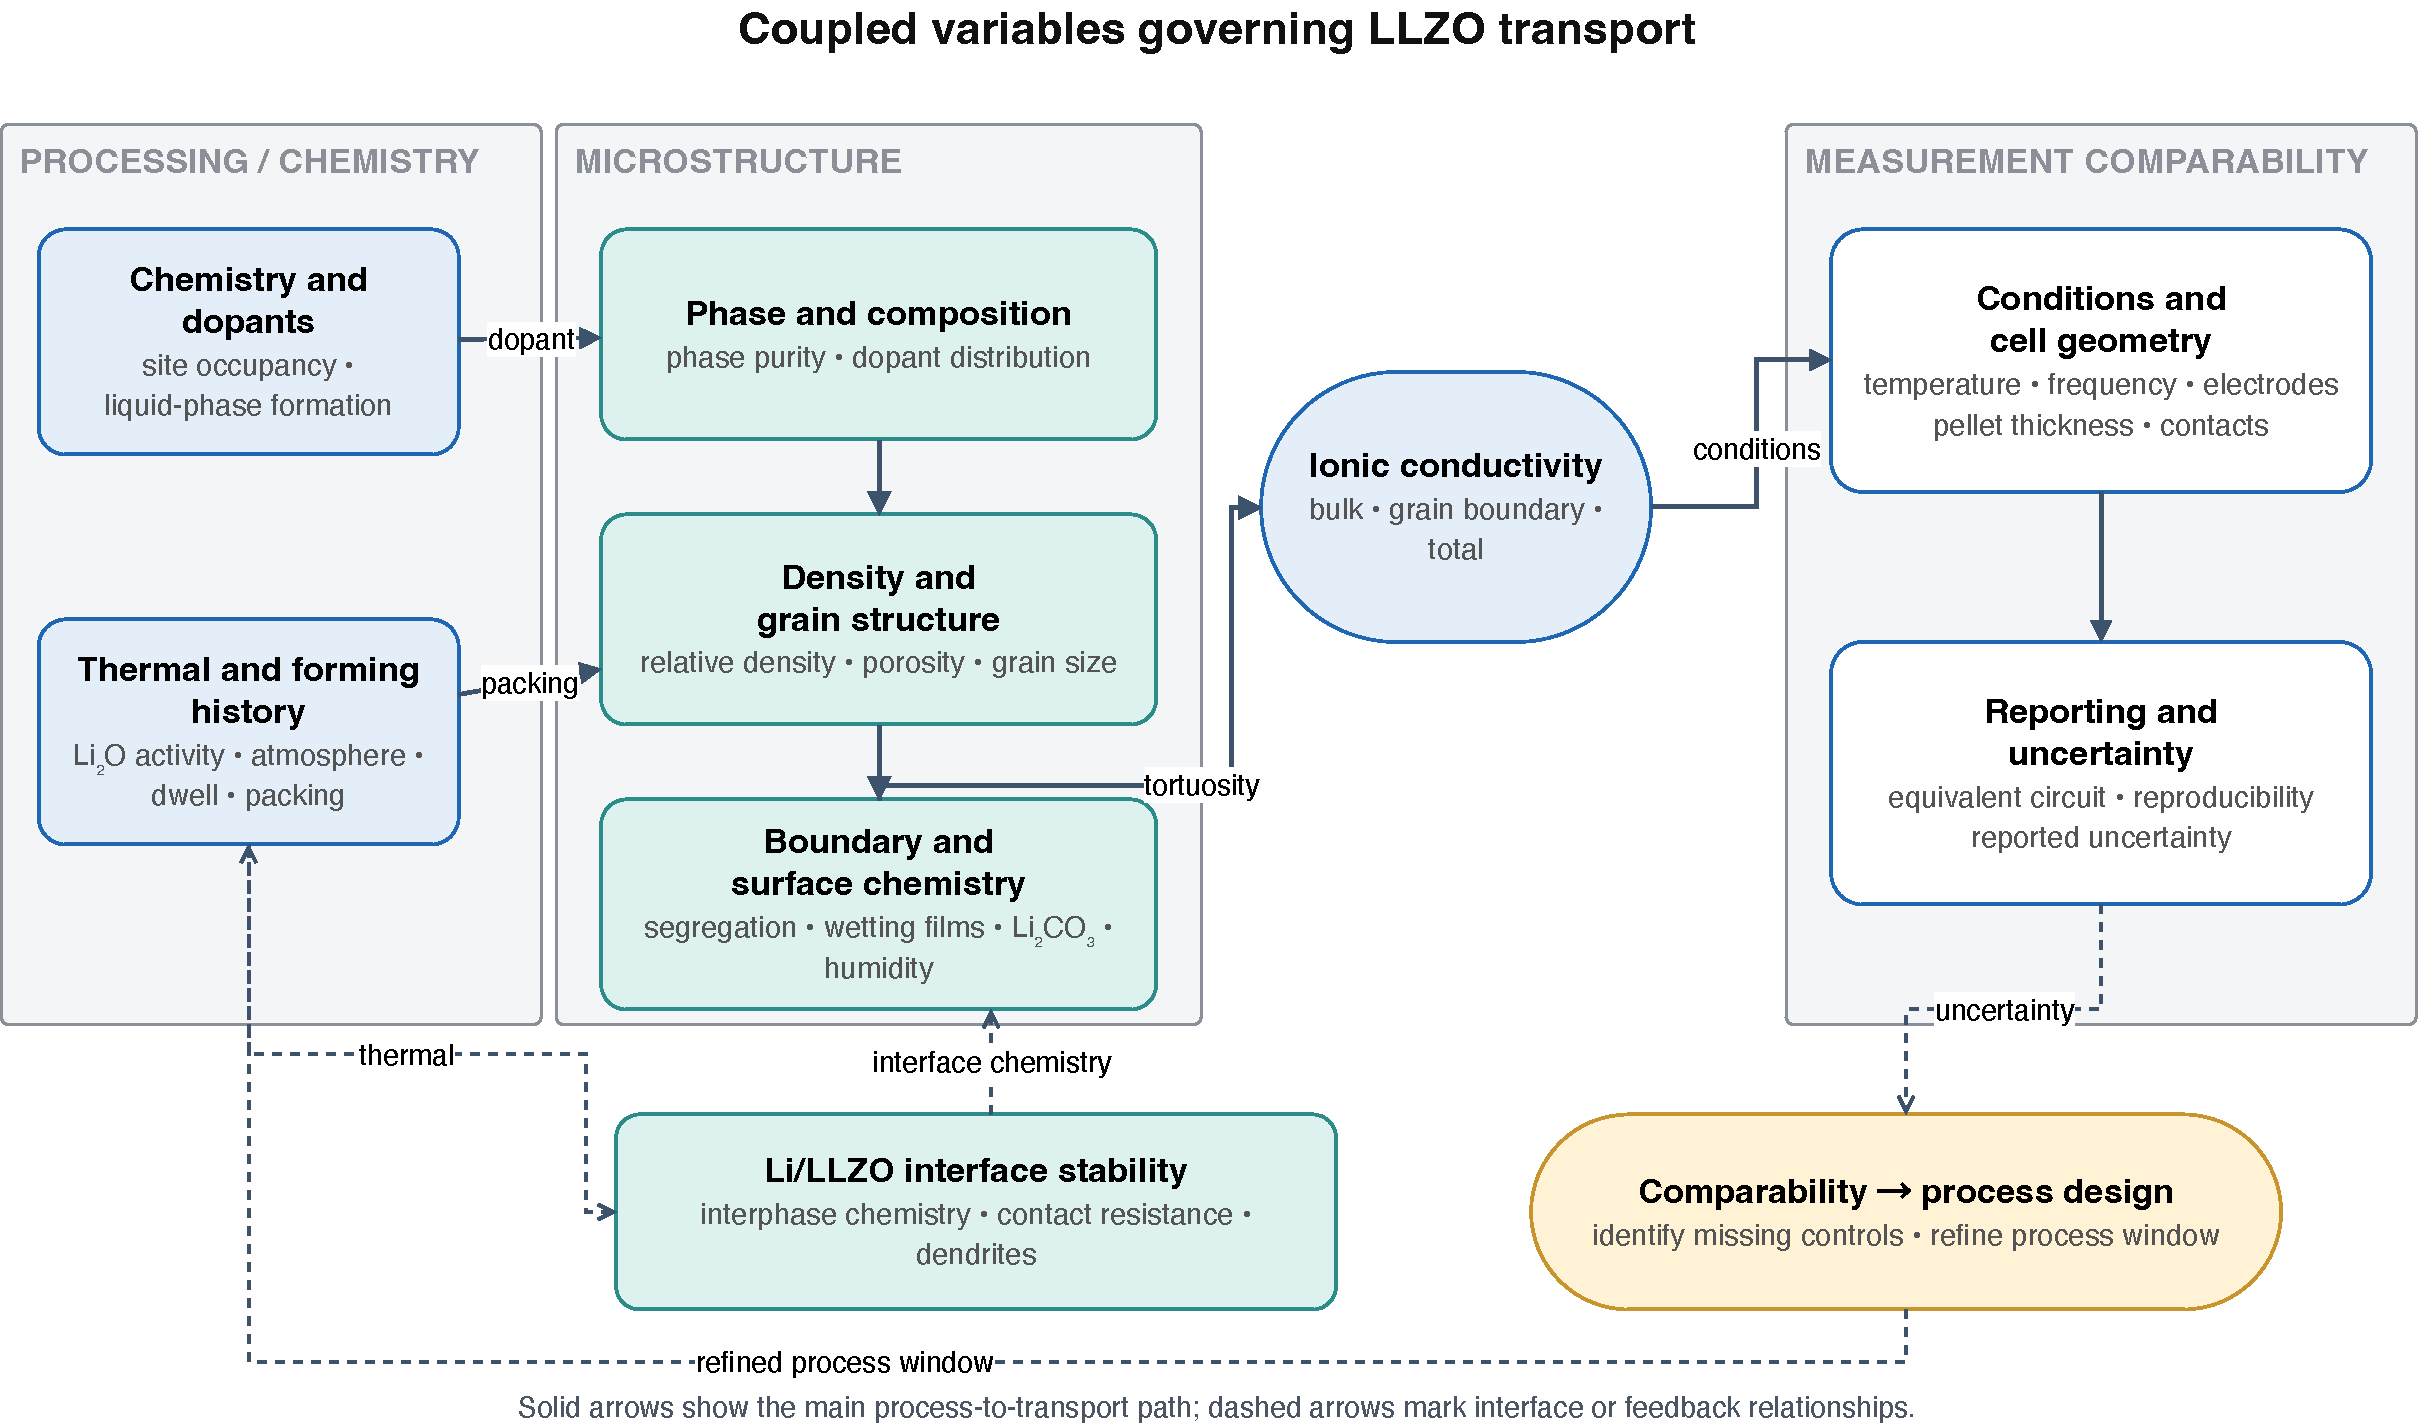
\includegraphics[width=0.98\linewidth]{../figures/pdf/fig3_coupled_variables.pdf}
  \caption{Coupled variables governing LLZO transport. Solid arrows show the main processing--structure--transport path; dashed arrows indicate interface and measurement feedbacks that constrain process design.}
  \label{fig:coupled-variables}
\end{figure}

\subsection{Limits of the present synthesis}

The source set contains many title- and abstract-level records, while detailed conditions are available for only a subset. Consequently, the review does not pool conductivity values or fit a meta-analysis. Near-neighbor garnets establish mechanisms but are not used to rank LLZO. Computational studies identify plausible pathways and descriptors, yet their predictions remain model-dependent until validated on matched specimens \cite{miyagawa2026raman,kulkarni2025machine}. Finally, the available local phase relations do not replace a composition--temperature--lithium-activity diagram; that absence is a measurement priority, not evidence that no such relation exists.
